\capitulo{3}{Conceptos teóricos}


En este capítulo se explicarán los conceptos teóricos subyacentes a todos los apartados del proyecto. Se afrontará en tres bloques: primero respecto a la teoría sobre la computación distribuida (\autoref{sec:tecdis}), otro sobre los flujos de datos (\autoref{sec:tecstream}) y,  por último, sobre la manipulación de imágenes (\autoref{sec:teccv}).

\section{Computación distribuida}\label{sec:tecdis}

Se denomina computación distribuida a las técnicas software para la gestión y el desarrollo sobre sistemas en los que sus componentes físicos y lógicos están separados y se comunican físicamente por red y lógicamente por paso de mensaje~\cite{wiki:computaciondistribuida}.

Es importante destacar que la computación distribuida no tiene una relación directa con la computación paralela~\cite{christos1994computational}, es decir, aquella que se ejecuta en diversos hilos de ejecución. 

La computación paralela no tiene por que ser distribuida ni viceversa. Sin embargo, es habitual que la computación distribuida sea paralela o el servicio se dé paralelamente a diferentes aplicaciones. Un caso típico de computación distribuida y paralela puede ser el de un servicio web. Cada conexión con el servidor es un hilo diferente de ejecución y los recursos necesarios para ofrecer el servicio (bases de datos, procesadores de información, etc.) estén distribuidos en la red.

Debido a que los sistemas que procesan \textit{Big Data} necesitan una gran cantidad de almacenamiento junto con herramientas que lo gestionen de la manera más eficiente posible, la mayoría de estos sistemas son distribuidos y paralelos.


\section{Flujos de datos}\label{sec:tecstream}

Un flujo de datos es una estructura de datos continua con elementos ilimitados que aparecen en orden secuencial y no permite acceso aleatorio a los datos. Por este motivo el conjunto de datos completo, ni siquiera una gran parte de los mismos, pueden ser incluidos en la memoria principal. Como los datos son continuos se pueden procesar individualmente, en bloques (también denominados \textit{chunks}) o por ventanas deslizantes. En la \autoref{fig:window} se puede observar el funcionamiento de las diferentes aproximaciones en el procesado del flujo.

\begin{figure}[H]
	\centering
	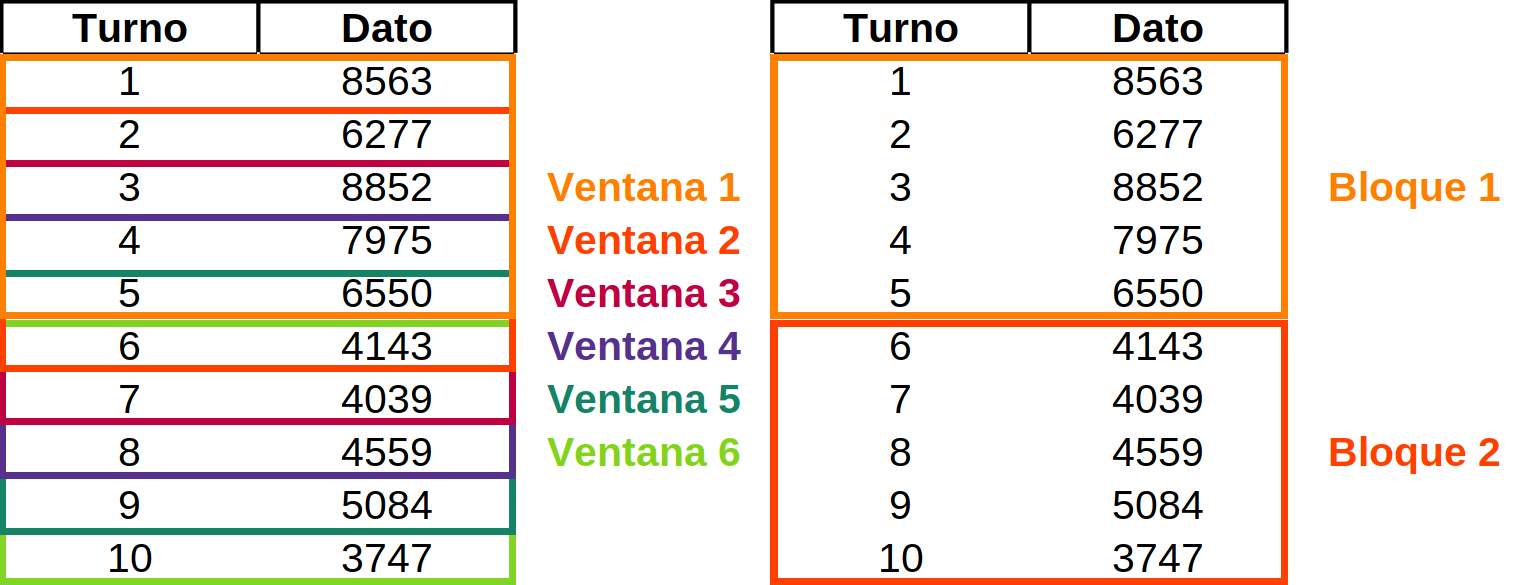
\includegraphics[width=0.8\textwidth]{ventanavsbloque}
	\caption{Diferentes aproximaciones para procesar un flujo de datos ejemplificado con el tamaño de cinco instancias. A la izquierda se puede observar el uso de ventanas deslizantes donde en cada turno se agrupan las últimas instancias. A la derecha se encuentra la aproximación por \textit{chunks} en el que se cogen grupos de cinco instancias sin compartirse entre bloques.}
	\label{fig:window}
\end{figure}


Por este motivo los algoritmos que procesan flujos de datos han de tener dos características principales~\cite{bifet2018machine}:

\begin{enumerate}
	\item deben procesar cada parte del flujo que reciban antes de que llegue la siguiente
	\item y deben procesar los datos usando una pequeña cantidad de memoria.
\end{enumerate}

Debido a esto, los algoritmos que se ejecutan sobre los flujos se suelen enfocar a soluciones aproximadas para minimizar el uso temporal y espacial. Además, si se aplican algoritmos cuyo comportamiento dependa de la evolución del flujo y el contenido del mismo cambia en sus características estadísticas, el programa debe poder adaptarse a estos cambios.

Para la adaptación de cambios existen dos aproximaciones principales: el uso de ventanas deslizantes, para que de este modo solo se tengan en cuenta los datos más recientes, y el uso de ventanas de decaimiento, en el que se da más peso a los datos más recientes. 

\subsection{Aplicaciones}

Los flujos de datos aparecen en multitud de entornos, principalmente en aquellos donde el tiempo real es más importante y los datos se generan continuamente.

Ejemplos de estas aplicaciones pueden ser~\cite{rodriguez2020flujos}:
\begin{itemize}
	\item Sensores en el \textit{Internet de las cosas} (\textit{IoT}),
	\item telecomunicaciones: llamadas, ubicación de los dispositivos $\ldots$,
	\item redes sociales: interacciones de los usuarios, tendencias $\ldots$,
	\item comercio electrónico: publicidad en tiempo real, actividad del usuario, detección de fraude $\ldots$,
	\item asistencia sanitaria: telemedicina, evolución de los pacientes $\ldots$,
	\item o epidemias y desastres naturales: evolución de una enfermedad, propagación vírica $\ldots$
\end{itemize}




\section{Procesamiento de imágenes}\label{sec:teccv}

A la hora de hacer procesamiento sobre vídeo, el fundamento principal es el procesamiento de los fotogramas que lo componen. Por tanto es importante entender cómo funcionan a nivel lógico las imágenes digitales, cómo operar con ellas y cómo procesarlas para obtener los mejores resultados.

\subsection{Definiciones}

\textbf{Imagen de 24 bits}: codificación habitual de las imágenes a color. Cada píxel se define como la combinación de tres enteros sin signo de 8 bits. La codificación (o espacio de color) necesaria para la visualización en monitores es la combinación de las capas de color roja, verde y azul, conocida como RGB, aunque también la BGR usada por openCV. 

\textbf{HSV}~\cite{wiki:hsv}: acrónimo del inglés de matiz, saturación y valor (\autoref{fig:hsv}). Consiste en un modelo de color basado en los componentes del mismo y representa una transformación no lineal del espacio de color RGB. El matiz, también conocido como tono, es el grado del ángulo respecto a la rueda de color. Representa un color único y algunos ejemplos son el rojo (0\grado), amarillo (60\grado) o verde (120\grado). La saturación representa la pureza del color entre el gris (valor mínimo) al color puro (valor máximo). El valor representa la luminosidad del color siendo el valor mínimo el color negro y el valor máximo el color con la saturación aplicada.

\begin{figure}
	\centering
	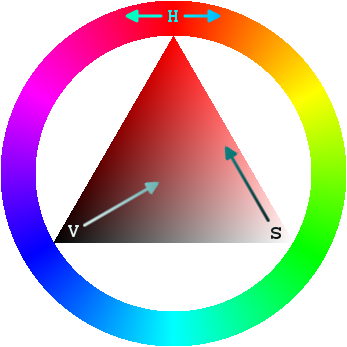
\includegraphics[width=0.5\textwidth]{Triangulo_HSV}
	\caption[Espacio de color HSV y la representación geométrica de cada componente.]{Espacio de color HSV y la representación geométrica de cada componente. Fuente: \href{https://commons.wikimedia.org/w/index.php?curid=1302915}{De Samus\_ - Trabajo propio, CC BY-SA 3.0}}
	\label{fig:hsv}
\end{figure}

\textbf{Histograma}~\cite{garrido2019opencv}: El histograma es una representación de cuántos píxeles hay para cada valor de intensidad. En él se puede ver información muy útil de la imagen como su brillo (media del histograma) o su contraste (diferencia entre el valor significativo\footnote{El valor mínimo y máximo tienden a ser siempre los mismos independientes del histograma (0 y 255 respectivamente), por eso se consideran los valores que tengan una presencia significativa, por ejemplo que sea al menos un 1\% de los valores.} máximo y mínimo). Los procesos de ajuste del brillo y contraste se pueden observar como transformaciones del histograma.

\subsection{Ajuste automático de brillo y contraste}
Para ajustar el brillo y contraste de una imagen $\textrm{I}$ hay que seleccionar dos valores $\alpha$ y $\beta$ que se deben aplicar sobre cada píxel de la imagen tal que la ecuación sea:
\begin{equation}
\textrm{I}'(x,y) = \alpha*\textrm{I}(x,y) + \beta\label{eq:brigh}
\end{equation}
Para hacer el proceso de manera automática es necesario encontrar los valores de $\alpha$ y $\beta$ adecuados. 
El procedimiento consiste en <<estirar>> una parte del histograma de la imagen de tal manera que el contenido seleccionado del mismo abarque todo el histograma, a esto se llama \textit{corte de alas} y va controlado por un parámetro que decide la posición del corte~(\autoref{fig:alphabeta}).

Por tanto, siendo $p$ el porcentaje mínimo de la frecuencia del \textit{valor} y $\vec{h}$ el histograma de la capa \textit{valor} de HSV, el proceso es el siguiente~\cite{pklab2017bright}:

\begin{enumerate}
	\item Se calcula la frecuencia acumulada de $\vec{h}$, lo definimos como el vector~$\vec{a}$.
	\item Se actualiza el valor de $p$ con $p = p*\frac{\mathbf{max}(\vec{a})}{100*2}$
	\item Se define un valor $g_{min}$ como el valor más alto de $\vec{a}$ que sea menor que $p$, también se define un valor $g_{max}$ como el valor más pequeño de $\vec{a}$ que sea mayor que $\mathbf{max}(\vec{a})-p$
	\item Se calcula el valor de $\alpha$ como $\alpha =  \frac{255}{g_{max} - g_{min}}$. (255 es el valor máximo permitido en la codificación 8 bits.)
	\item Se calcula el valor de $\beta$ como $\beta = -g_{min} * \alpha$.
\end{enumerate}

\begin{figure}[h]
	\centering
	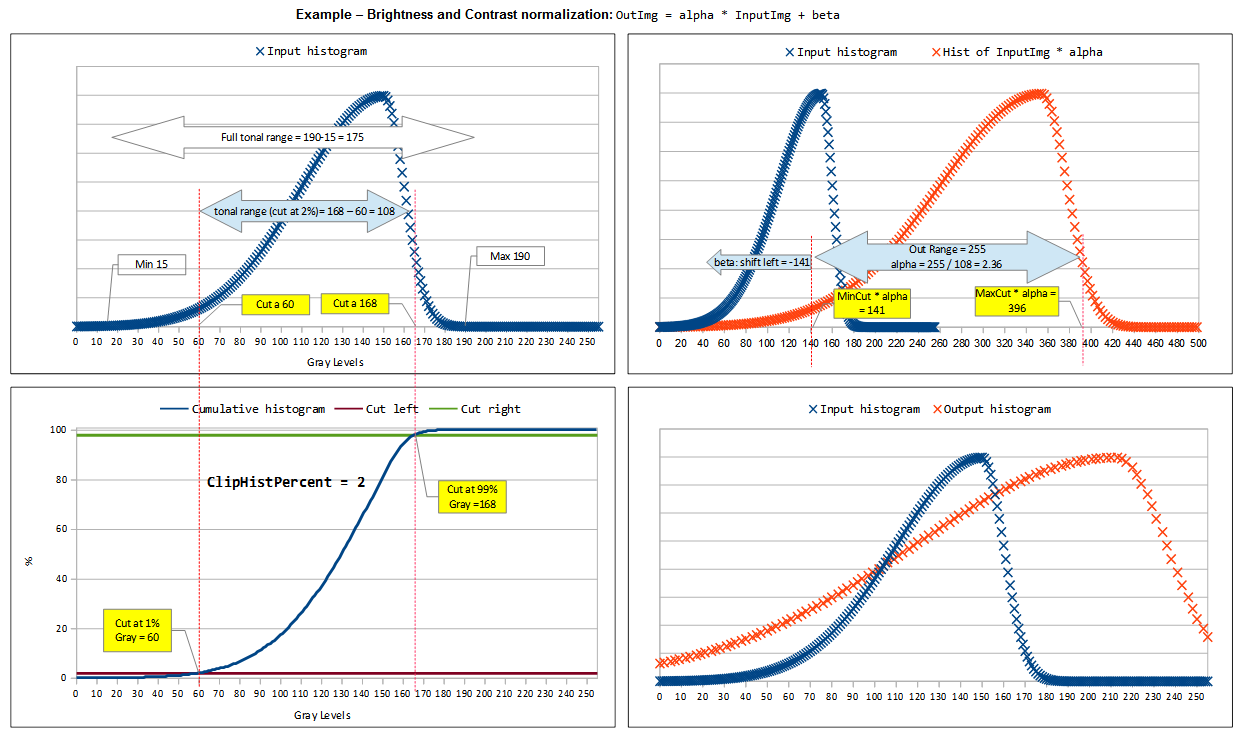
\includegraphics[width=1\textwidth]{alphabetaImageProcessing}
	\caption[Ejemplo visual del cálculo de $\alpha$ y $\beta$ para una imagen]{Ejemplo visual del cálculo de $\alpha$ y $\beta$ para una imagen. Fuente: \href{https://answers.opencv.org/question/75510/how-to-make-auto-adjustmentsbrightness-and-contrast-for-image-android-opencv-image-correction/}{De PKLab - en opencv.org}}
	\label{fig:alphabeta}
\end{figure}

En el caso de que se quisiera dejar el mismo brillo y solo cambiar el contraste, el valor de $\alpha$ a aplicar en la ecuación \eqref{eq:brigh} será 1, en caso opuesto el valor de $\beta$ deberá ser 0.

